%---------- Quarto Capítulo: Desenvolvimento ----------

\chapter{Desenvolvimento} %10 --- 20 pags

\section{Ferramentas Utilizadas}
\subsection{Ambientes de Desenvolvimento}
\subsection{Repositório}

\section{Ferramentas Desenvolvidas}
\subsection{Block}
\subsection{Blur}
\subsection{NetSim}

A ferramenta Netsim foi desenvolvida buscando simular degradações ocasionadas pelo processo de decodificação de um streaming de vídeo onde houve perda de informação nas camadas de transporte, rede ou enlace. O Netsim desconsidera, portanto, os artefados decorrentes do processo de codificação e encapsulamento do vídeo.

As simulações efetuadas pela ferramenta atuam sobre vídeos encapsulados no formato MPEG Transport Stream, conforme definido em \cite{} %TODO referencia para ITU-T Rec. H.222.0
e consistem no descarte controlado de porções de informação. 
A entidade de dados a ser descartada pode ser tanto um único TS quanto o equivalente a um pacote UDP da camada de transporte, o qual comporta usualmente sete unidades TS.
O descarte é controlado precisamente por meio de um arquivo de configuração fornecido como paramêtro ao programa, podendo este ser gerado pela ferramenta Raffle descrita em \ref{}. %TODO referencia pra raffle.
Este arquivo de configuração deve conter duas colunas com valores numéricos inteiros. 
Cada linha será processada sequencialmente, sendo que o primeiro número indica quantas entidades serão transportadas com sucesso e o segundo quantas serão descartadas. 
A Figura \ref{fig:netsim} ilustra a sequência.

\begin{figure}[!htb]
	\centering
	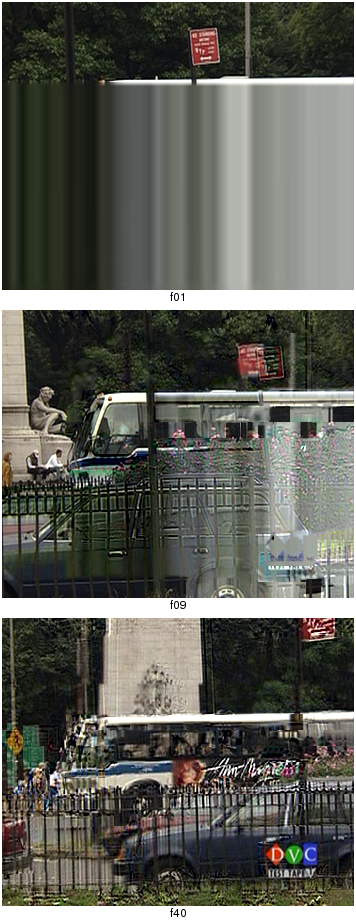
\includegraphics[width=0.9\textwidth]{./imgs/netsim.png}
	\caption{Ilustração do arquivo de configuração de descartes da ferramenta Netsim.}
	\label{fig:netsim}
	\fonte{Autoria Própria.}
\end{figure}

Neste caso, \emph{A} e \emph{C} indicam o número de entidades que atingem seu destino com sucesso e \emph{B} e \emph{D} indicam quantas serão descartadas. 
Sendo assim o streaming de vídeo da Figura \ref{fig:netsim}  teria seus primeiros \emph{A} pacotes intactos, seguidos de \emph{B} perdidos, mais \emph{C} pacotes intactos e ainda \emph{D} perdidos novamente.

\begin{description}
	\item[\texttt{--input}] \hfill \\
		Define o caminho(absoluto ou relativo) e arquivo do vídeo a ser processado pela simulação.
	\item[\texttt{--output}] \hfill \\
		Define o caminho(absoluto ou relativo) e arquivo onde será armazenado o vídeo resultante.
	\item[\texttt{--ts}] \hfill \\
		(Opcional) Se presente, a entidade de descarte considerada é um TS, caso contrário a unidade é um pacote UDP.
	\item[\texttt{--raffle}] \hfill \\
		Indica o caminho(absoluto ou relativo) e arquivo a ser usado como configuração de descartes.
\end{description}

\subsection{Raffle}
\subsection{Metric}

A ferramenta Metric se trata da implementação de três métricas objetivas, as mesma encontradas na implementação do SASQV:

\begin{itemize}
	\item MSE
	\item PSNR
	\item MSSIM
\end{itemize}

Implementada em C++, também na forma de uma ferramenta \emph{stand-alone}, seu funcionamento é baseado em verificar disparidades entre dois vídeos fornecidos seguindo uma das métricas implementadas e fornecer um resultado numérico. 
Os vídeos a serem comparados devem possuir as mesmas dimensões e número de frames para serem passíveis de comparação. 
A ferramenta Metric pode receber os seguintes parametros:

\begin{description}
	\item[\texttt{--input}] \hfill \\
		Define o caminho(absoluto ou relativo) e arquivo onde um dos vídeos a serem comparados se encontra.
	\item[\texttt{--reference}] \hfill \\
		Define o caminho(absoluto ou relativo) e arquivo onde o segundo vídeo a ser comparado se encontra.
	\item[\texttt{--size}] \hfill \\
		Define as dimensões (em pixels) dos vídeos a serem comparados. Deve ser fornecida no formato 'largura'x'altura'.
	\item[\texttt{--metric}] \hfill \\
		Define qual métrica será utilizada na comparação entre vídeos, sendo uma string entre MSE, PSNR ou MSSIM.
	\item[\texttt{--window}] \hfill \\
		Define qual o tamanho da janela (em pixels) a ser usado se a métrica adotada for MSSIM.
\end{description}

\section{Interface Gráfica}
\subsection{Sessão}
\subsection{Ferramentas}
\subsection{Resultados}
\subsection{Configurações}
\subsection{Ajuda}

\section{Diagramas de Classes}

\section{Diagramas de Sequências}
\section{Considerações}
